\chapter{\ifproject%
\ifcpe โครงสร้างและขั้นตอนการทำงาน\else Project Structure and Methodology\fi
\else%
\ifcpe โครงสร้างของโครงงาน\else Project Structure\fi
\fi
}

ในบทนี้จะกล่าวถึงหลักการ และการออกแบบระบบ

\makeatletter

% \renewcommand\section{\@startsection {section}{1}{\z@}%
%                                    {13.5ex \@plus -1ex \@minus -.2ex}%
%                                    {2.3ex \@plus.2ex}%
%                                    {\normalfont\large\bfseries}}

\makeatother
%\vspace{2ex}
% \titleformat{\section}{\normalfont\bfseries}{\thesection}{1em}{}
% \titlespacing*{\section}{0pt}{10ex}{0pt}



\section{โครงสร้างของระบบ}



\subsection{Database Design}
  \begin{center}
    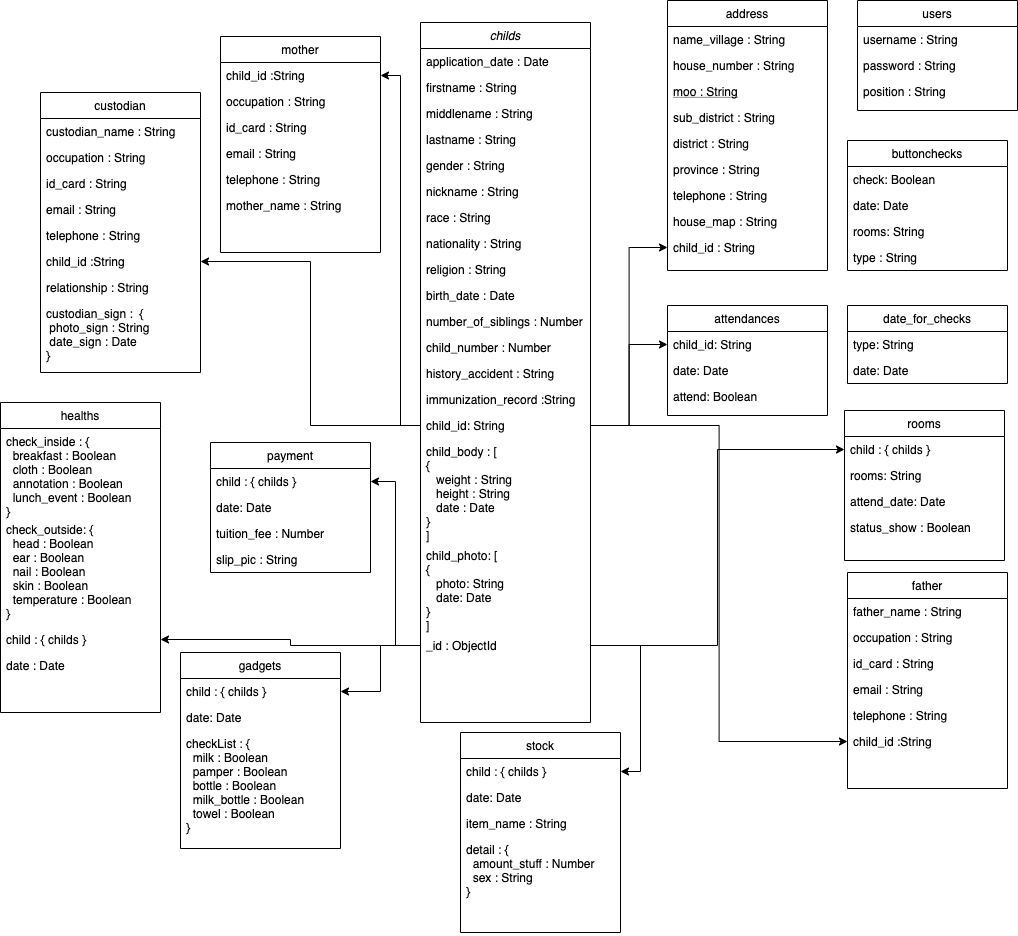
\includegraphics[width=\linewidth]{images/databaseDiagram.png}
    \CIreply{รูปเล็ก มองไม่เห็น ควรทำเป็น landscape figure}
  \end{center}
    
  ประเภทของฐานข้อมูลที่ใช้เป็นแบบ \CI{NOSQL}{check spelling} รายละเอียดของ Collection ในฐานข้อมูลของโครงงานนี้ มีดังนี้
  \begin{itemize}
    \item childs เก็บข้อมูลเกี่ยวข้องกับเด็กทั้งหมด 
    \item father เก็บข้อมูลส่วนตัวของพ่อเด็ก
    \item mother เก็บข้อมูลส่วนตัวของแม่เด็ก
    \item custodian เก็บข้อมูลส่วนตัวของผู้ปกครองเด็ก
    \item address เก็บข้อมูลที่อยู่ของเด็ก
    \item users เก็บ Username Password สำหรับเข้าสู่ ระบบจัดการ Nursery 
    \item buttonchecks เก็บข้อมูลสำหรับใช้เช็คว่าวันนี้มีการเช็คชื่อไปยัง
    \item date\_for\_checks เก็บวันที่ใช้เช็คชื่อย้อนหลัง
    \item rooms เก็บข้อมูลการเรียนของเด็กในห้องต่างๆ
    \item attendances เก็บข้อมูลการเช็คชื่อทั้งหมด
    \item gadgets เก็บข้อมูลการเช็คอุปกรณ์ของเด็กทั้งหมด
    \item healths เก็บข้อมูลการเช็คสุขภาพของเด็กทั้งหมด
    \item stock เก็บข้อมูลของใช้ทั้งหมดของเด็กใน Nursery 
    \item payment เก็บข้อมูลประวัติการโอนเงินค่าเล่าเรียนของผู้ปกครองเด็ก

  \end{itemize}
\CIreply{ลงรายละเอียดในแต่ละ table ให้มากกว่านี้ และอธิบายลูกศรที่ปรากฎในแผนภาพด้วย}

\subsection{XD Design}
\begin{enumerate}
  \item RegisterPage คือ หน้าแบบฟอร์มในการลงทะเบียนเด็กในการเข้าเรียน Nursery รูปที่~\ref{fig:register}
  \item  ProfilePage  คือ หน้าที่ใช้ในการจัดการกับประวัติส่วนตัวของเด็ก สามารถแสดงข้อมูลและแก้ไขข้อมูลของเด็กแต่ละคนได้ รูปที่~\ref{fig:Profile} \ref{fig:ProfileTwo} \ref{fig:UpdateProfile}
  \item  Attendance คือ หน้าเช็คชื่อเด็กรายวัน รูปที่~\ref{fig:Attendance} \ref{fig:CheckAttendance}
  \item  Health คือ หน้าเช็คสุขภาพเด็กรายวัน รูปที่~\ref{fig:Health} \ref{fig:CheckHealth}
  \item  Gadget คือ หน้าเช็คของเด็กรายวัน รูปที่~\ref{fig:Gadget} \ref{fig:CheckGadget}
  \item  Stock คือ หน้าจัดการของใช้สำหรับเด็กทั้งหมดใน Nursery รูปที่~\ref{fig:Stock} \ref{fig:CheckStock}
  \item  Payment คือ หน้าที่ใช้จัดการกับใบเสร็จ  ประวัติการจ่ายเงินค่าเล่าเรียน รูปที่~\ref{fig:Payment}
\end{enumerate}

\begin{figure}
  \begin{center}
  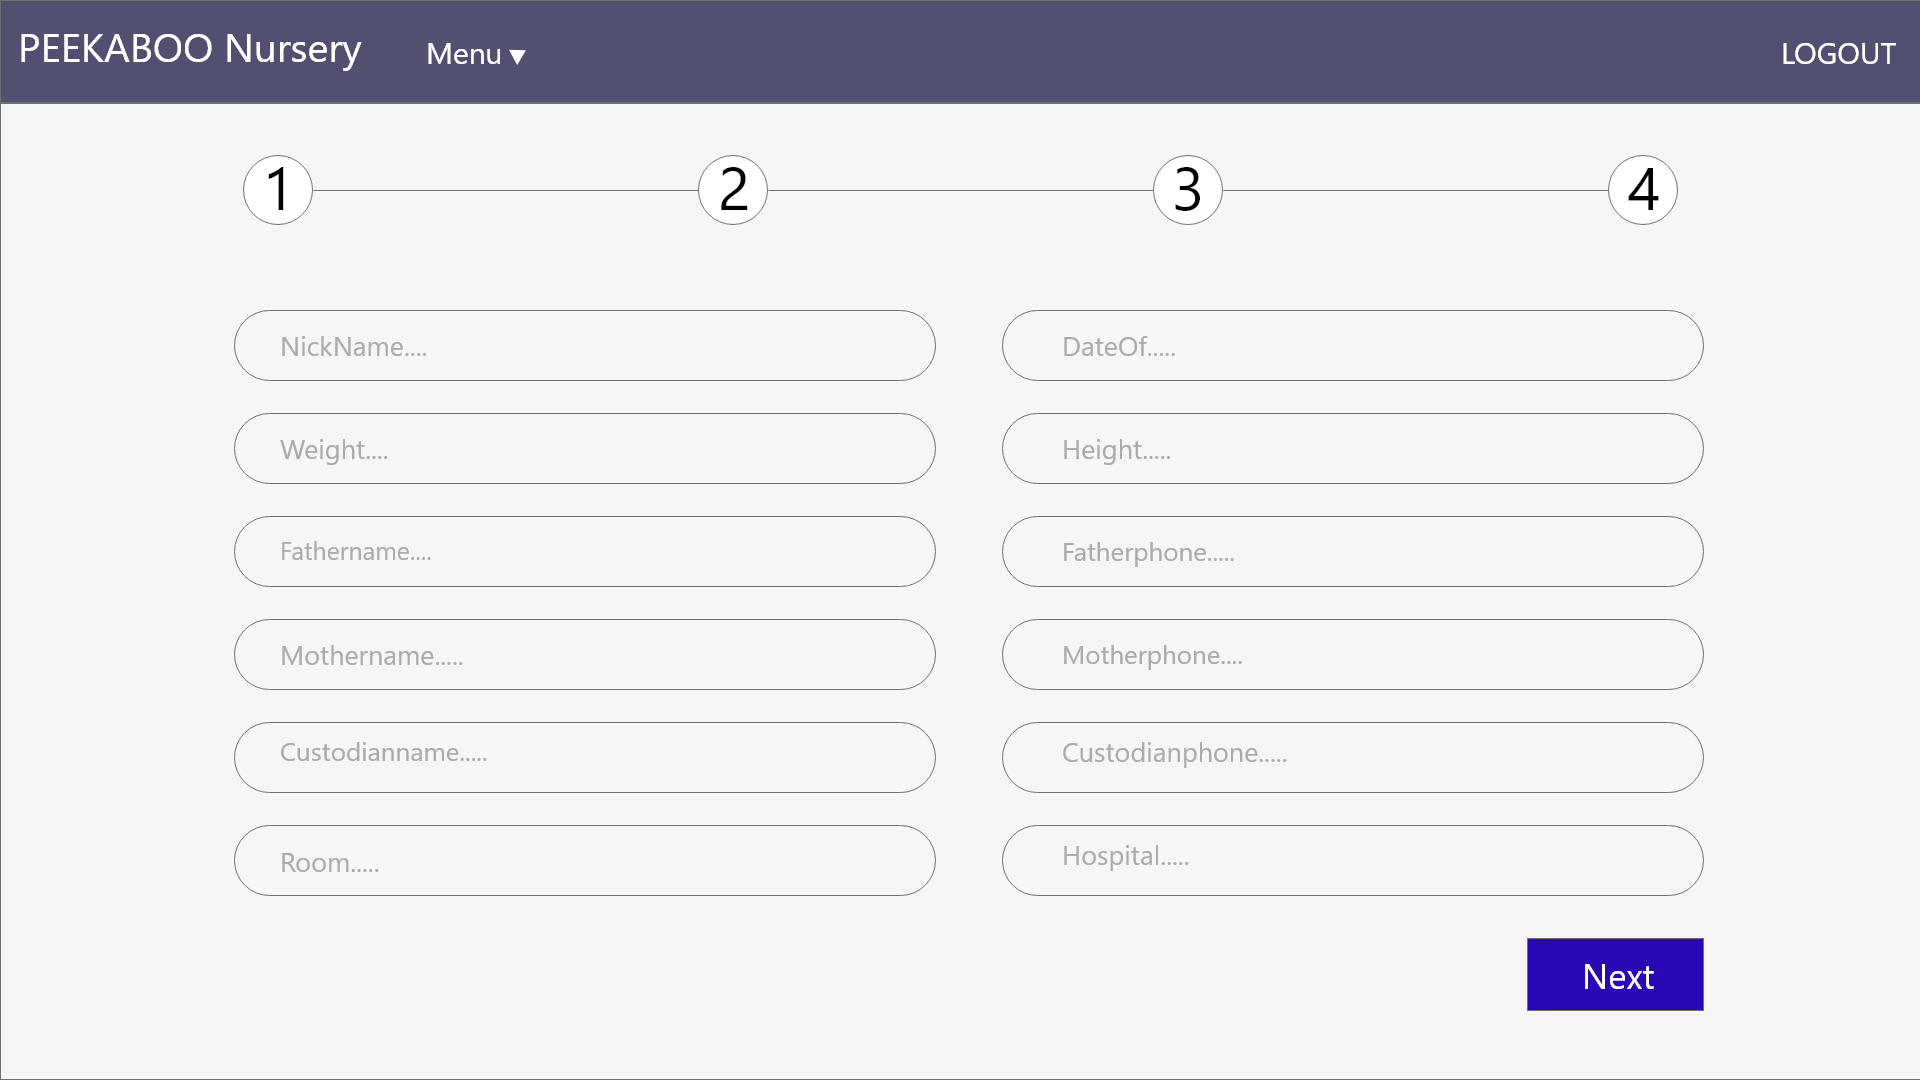
\includegraphics[width=\linewidth]{images/registerPage.png}
  \end{center}
  \caption[Poem]{Register Page}
  \label{fig:register}
  \end{figure}

\begin{figure}
  \begin{center}
  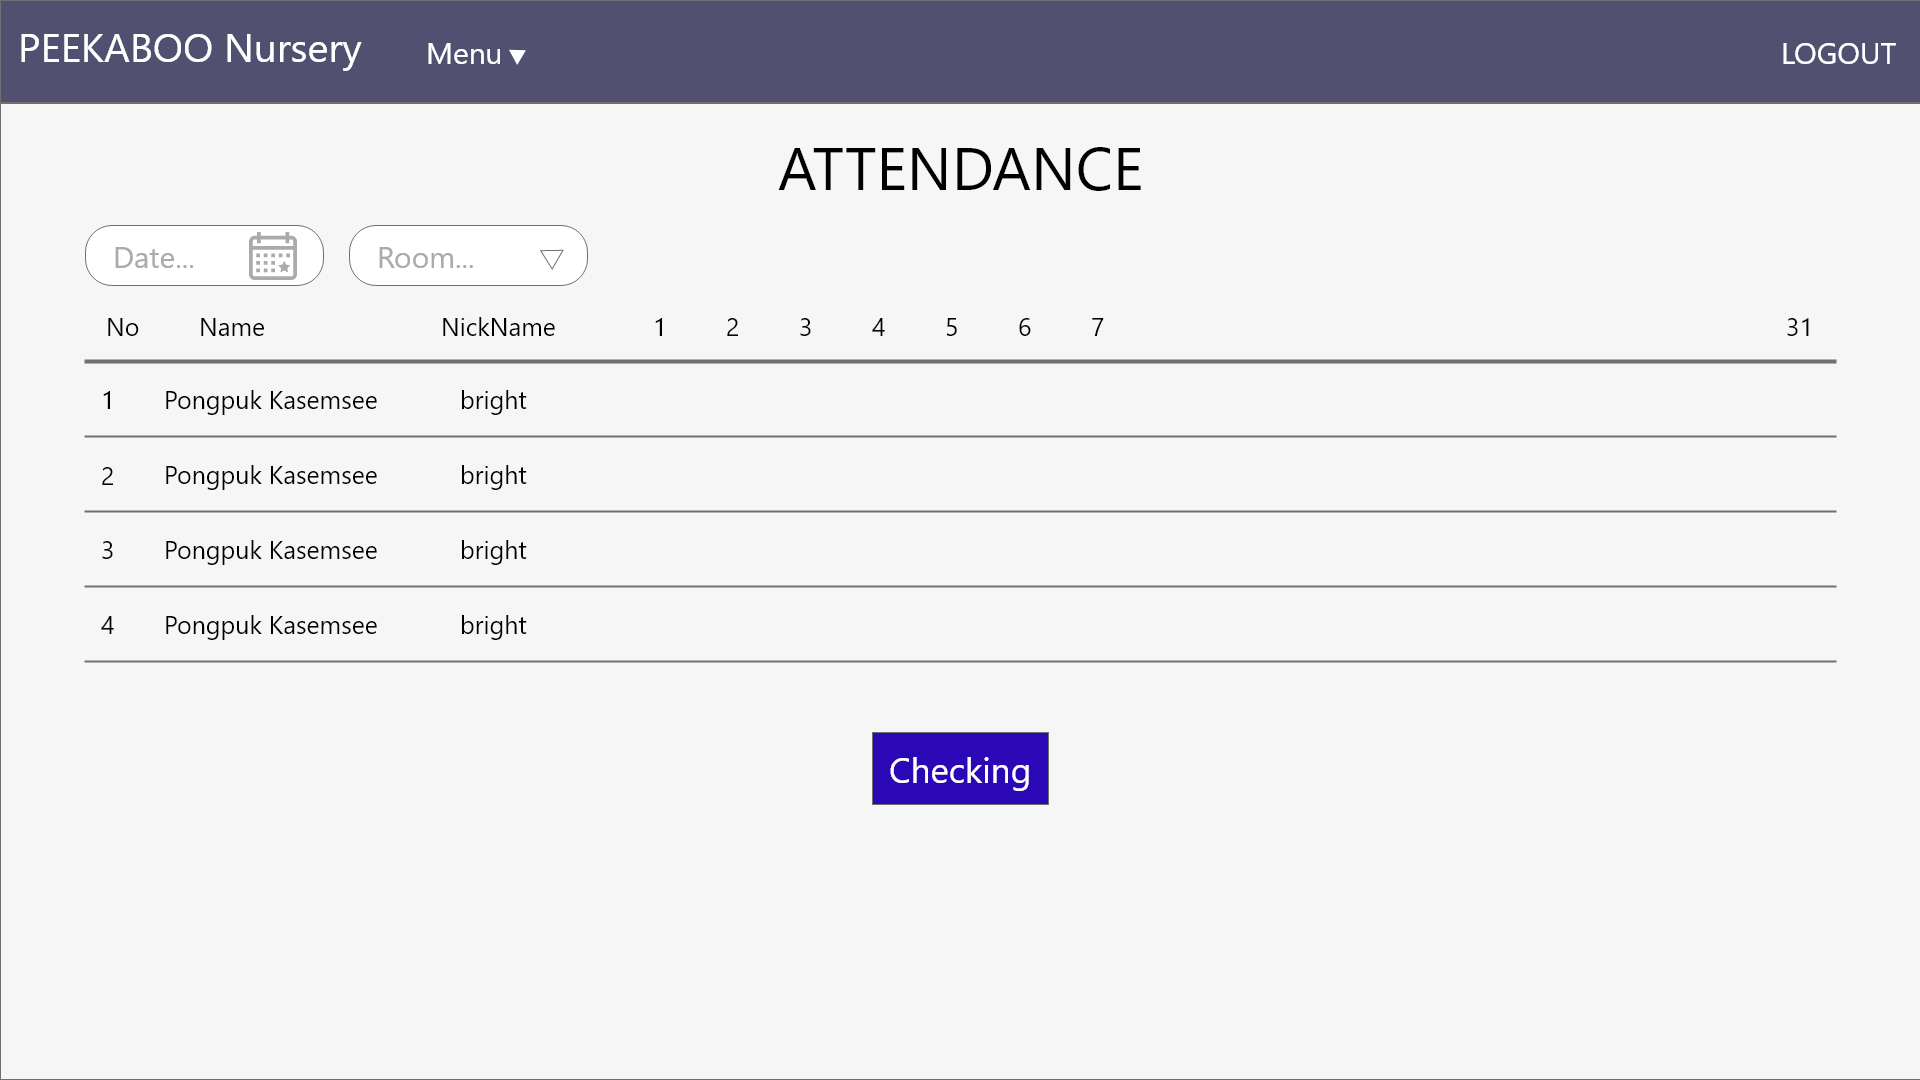
\includegraphics[width=\linewidth]{images/AttendancePage.png}
  \end{center}
  \caption[Poem]{Attendance Page}
  \label{fig:Attendance}
  \end{figure}

\begin{figure}
  \begin{center}
  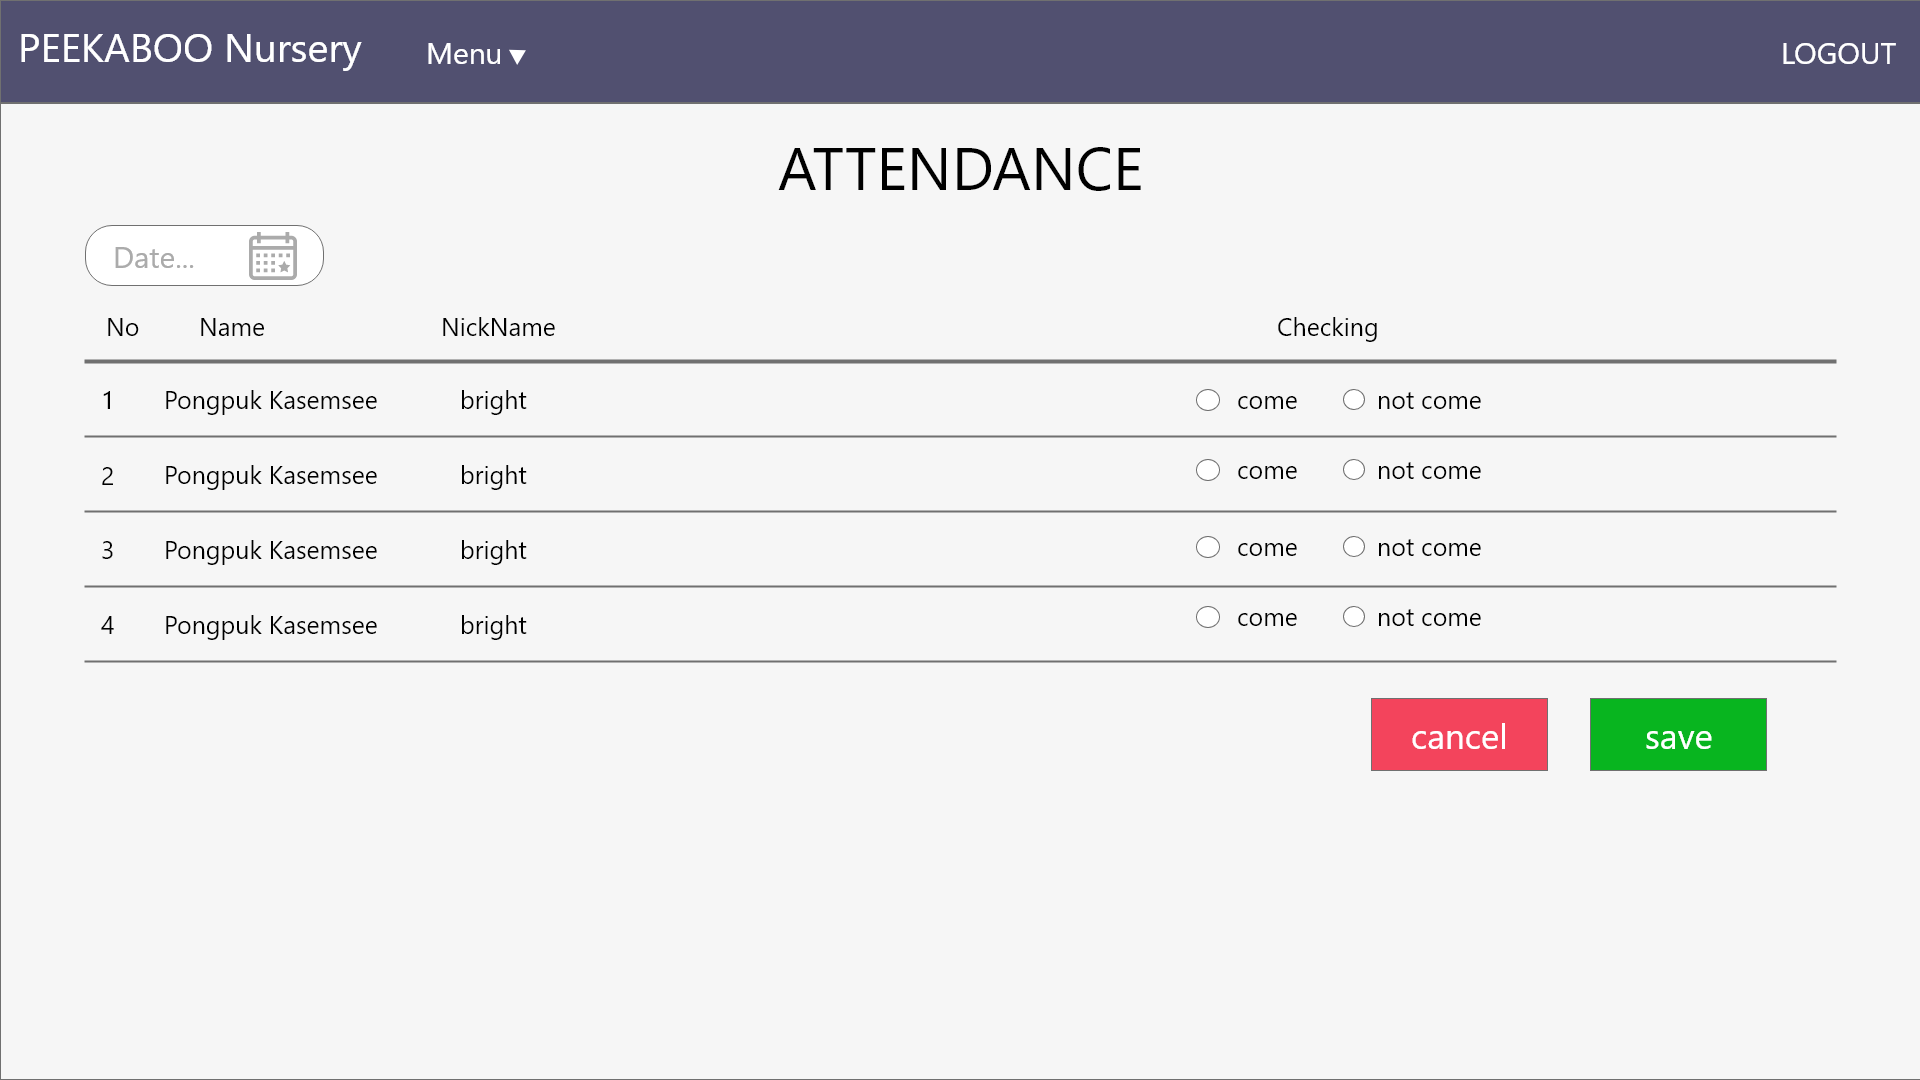
\includegraphics[width=\linewidth]{images/AttendancePageChecking.png}
  \end{center}
  \caption[Poem]{Check Attendance Page}
  \label{fig:CheckAttendance}
  \end{figure}

\begin{figure}
  \begin{center}
  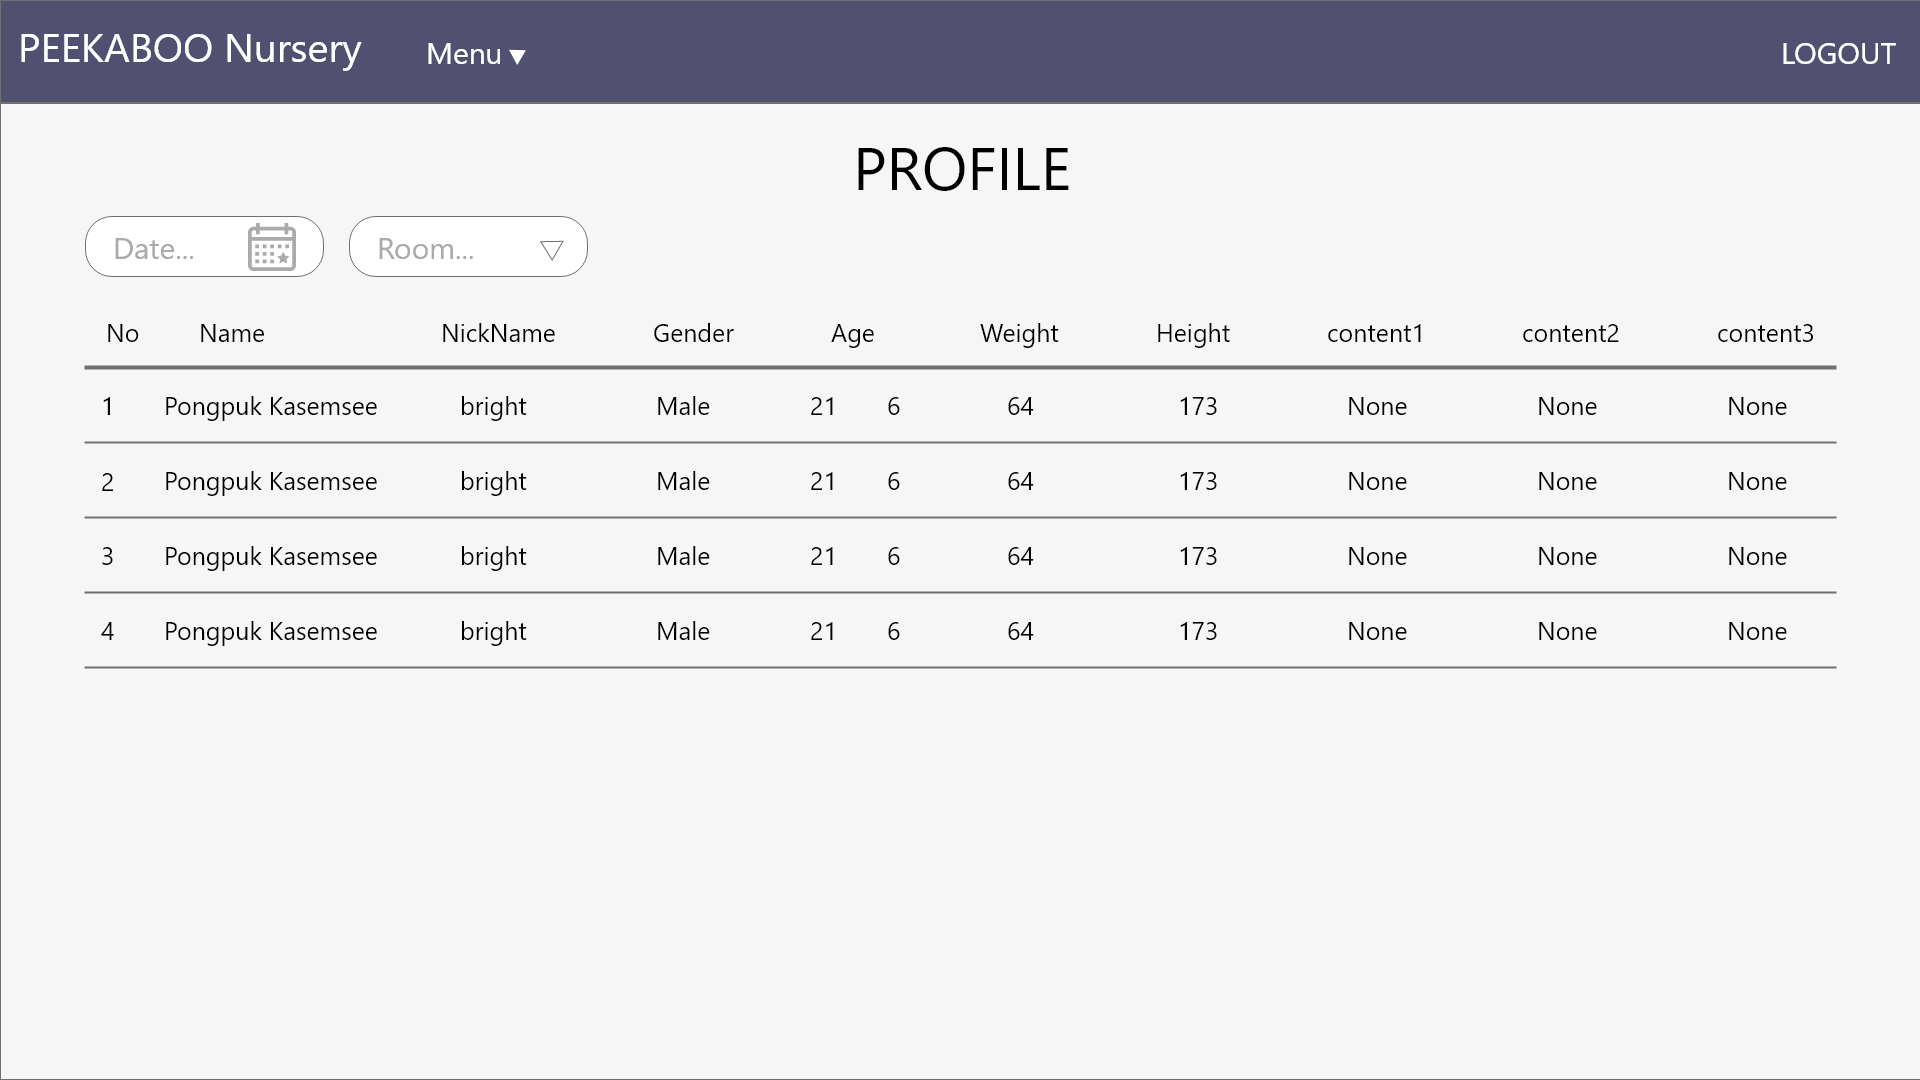
\includegraphics[width=\linewidth]{images/ProfileOnePage.png}
  \end{center}
  \caption[Poem]{Profile Page}
  \label{fig:Profile}
  \end{figure}

\begin{figure}
  \begin{center}
  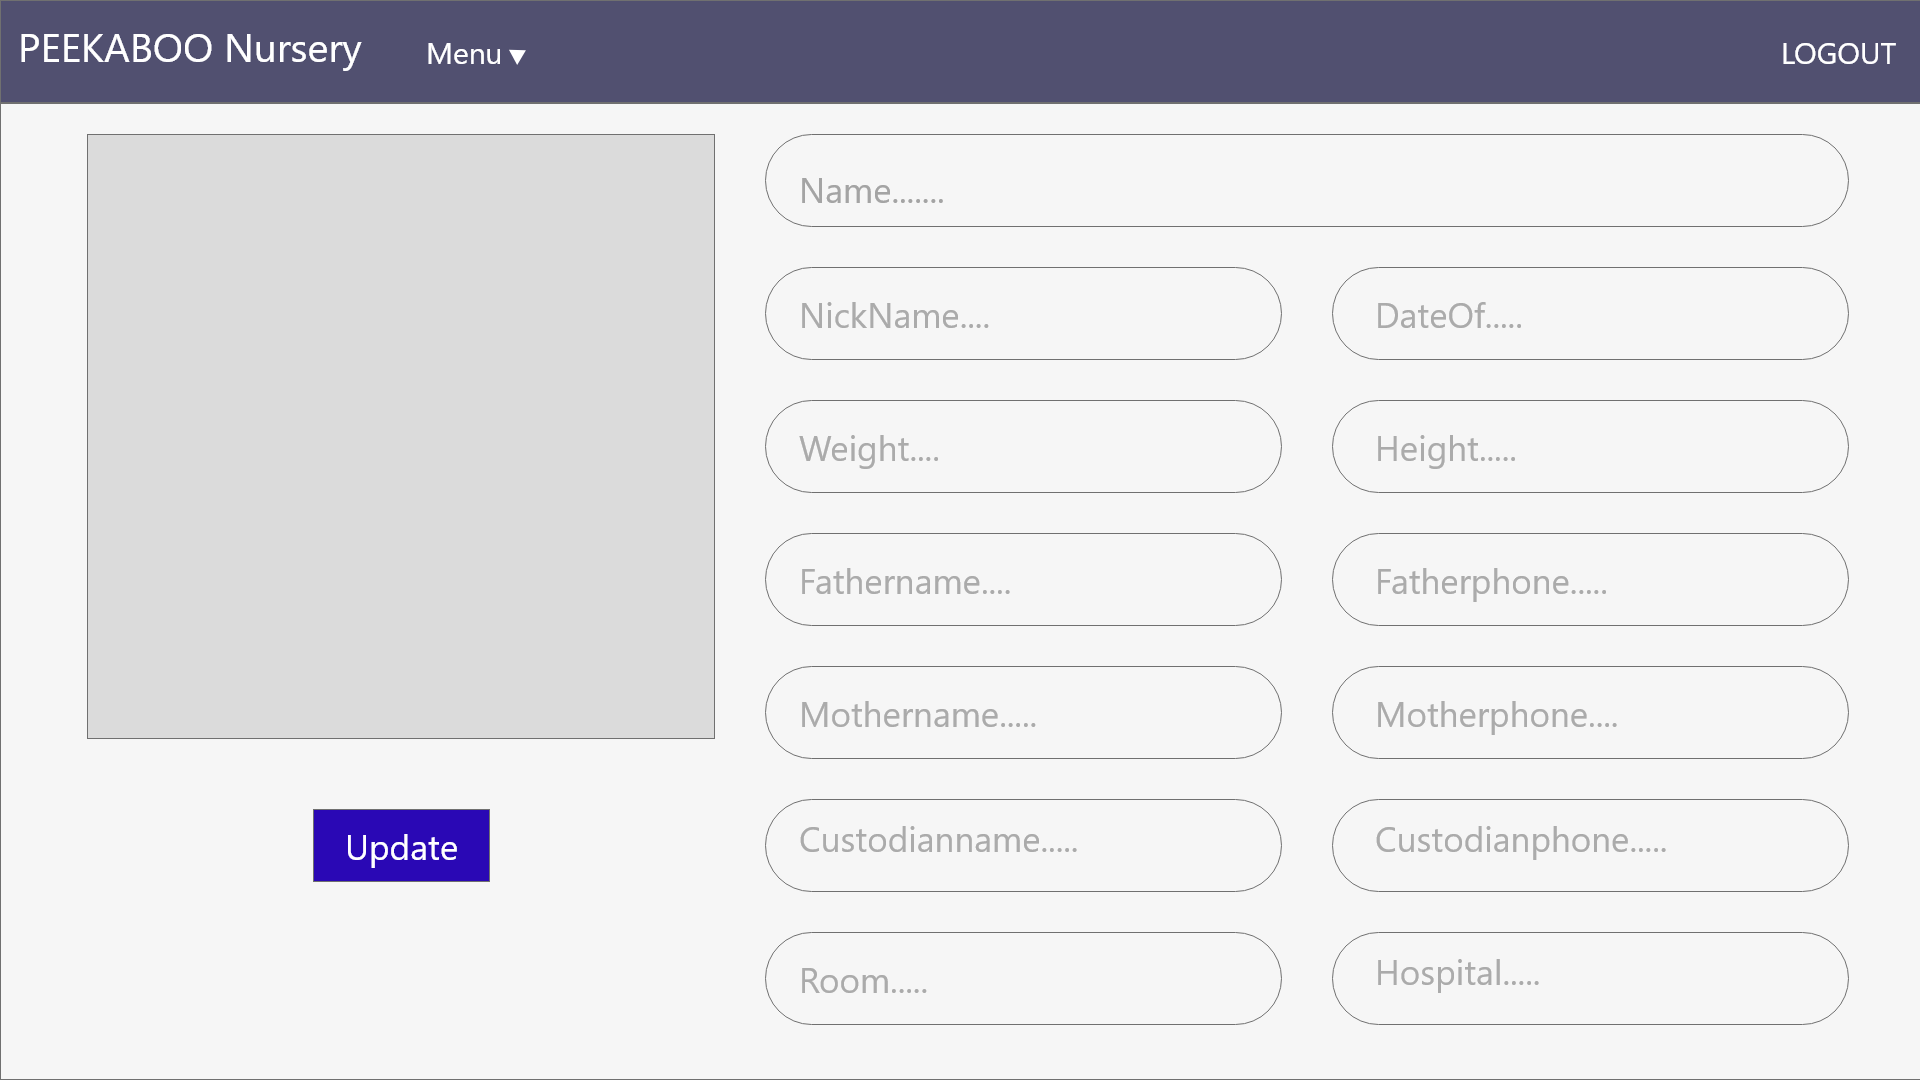
\includegraphics[width=\linewidth]{images/ProfileTwoPage.png}
  \end{center}
  \caption[Poem]{Profile Page}
  \label{fig:ProfileTwo}
  \end{figure}

\begin{figure}
  \begin{center}
  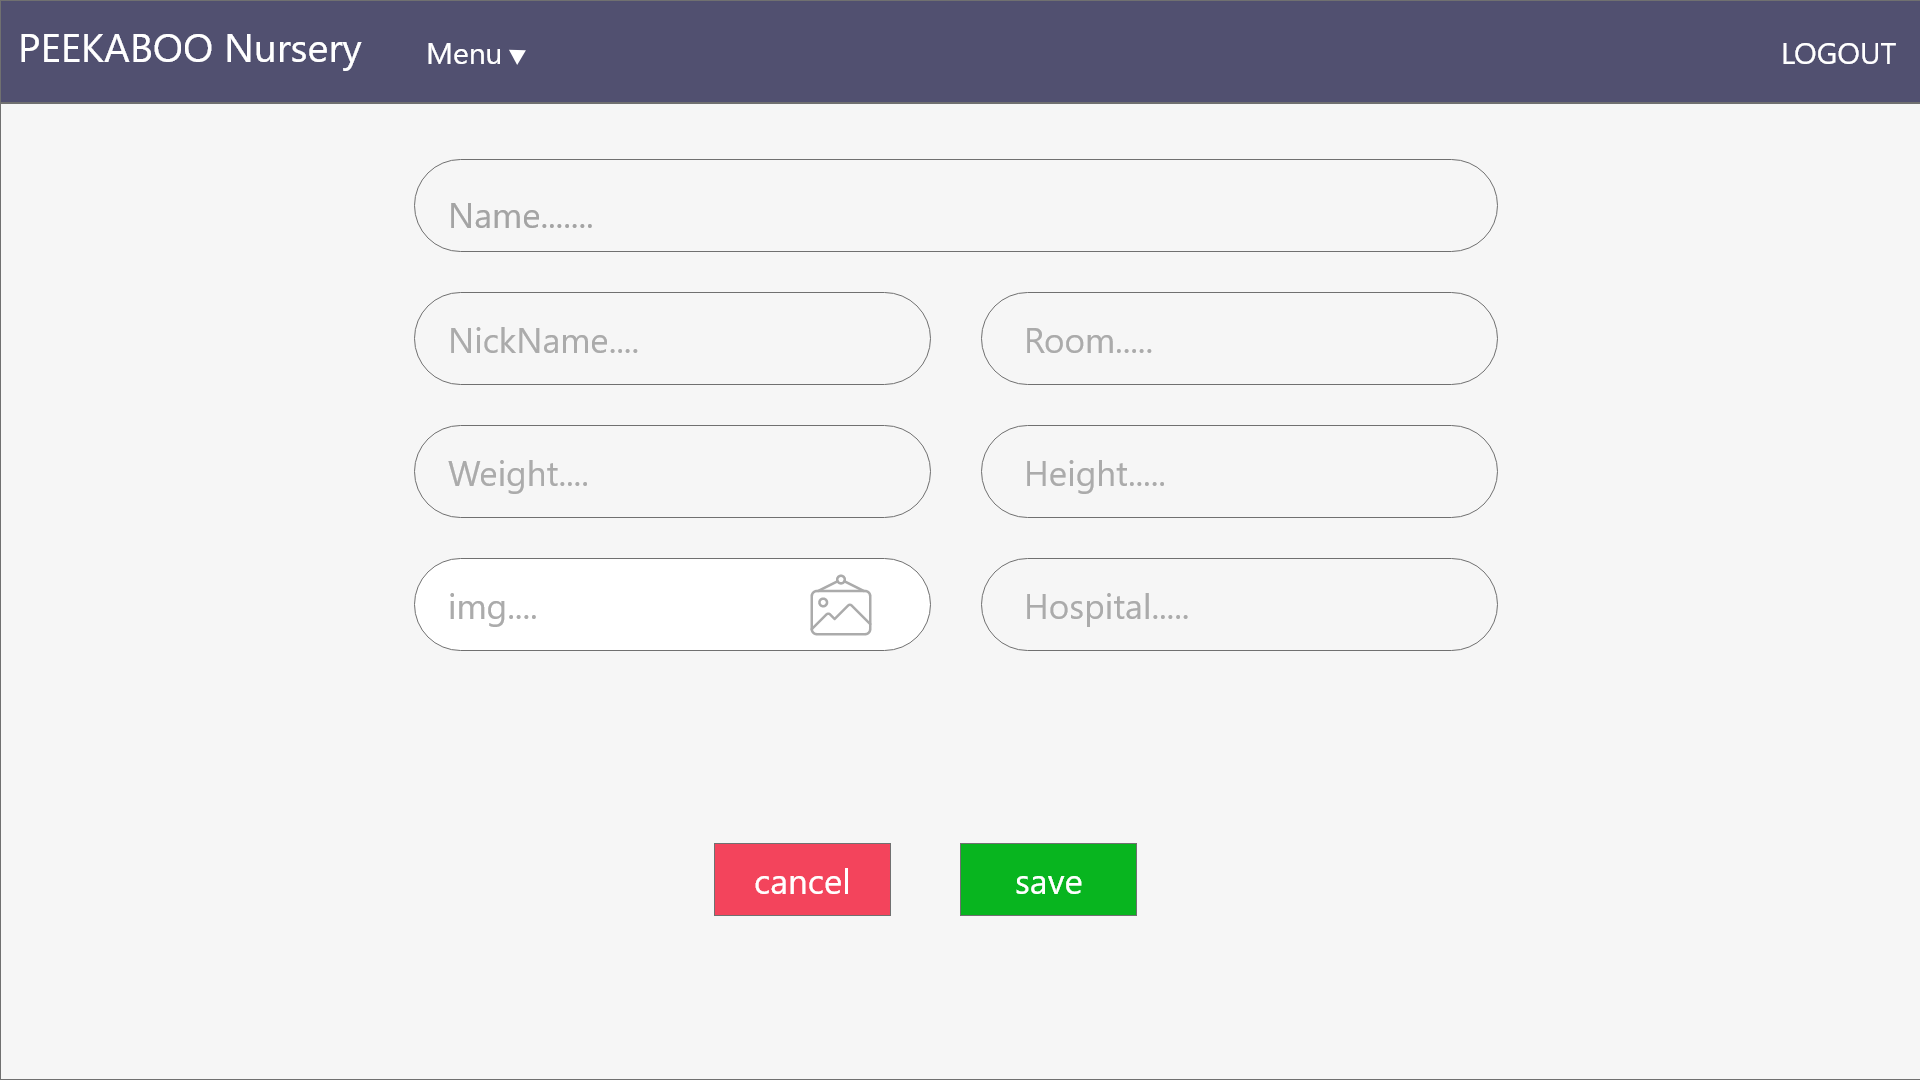
\includegraphics[width=\linewidth]{images/updateprofilePage.png}
  \end{center}
  \caption[Poem]{Update Profile Page}
  \label{fig:UpdateProfile}
  \end{figure}

\begin{figure}
  \begin{center}
  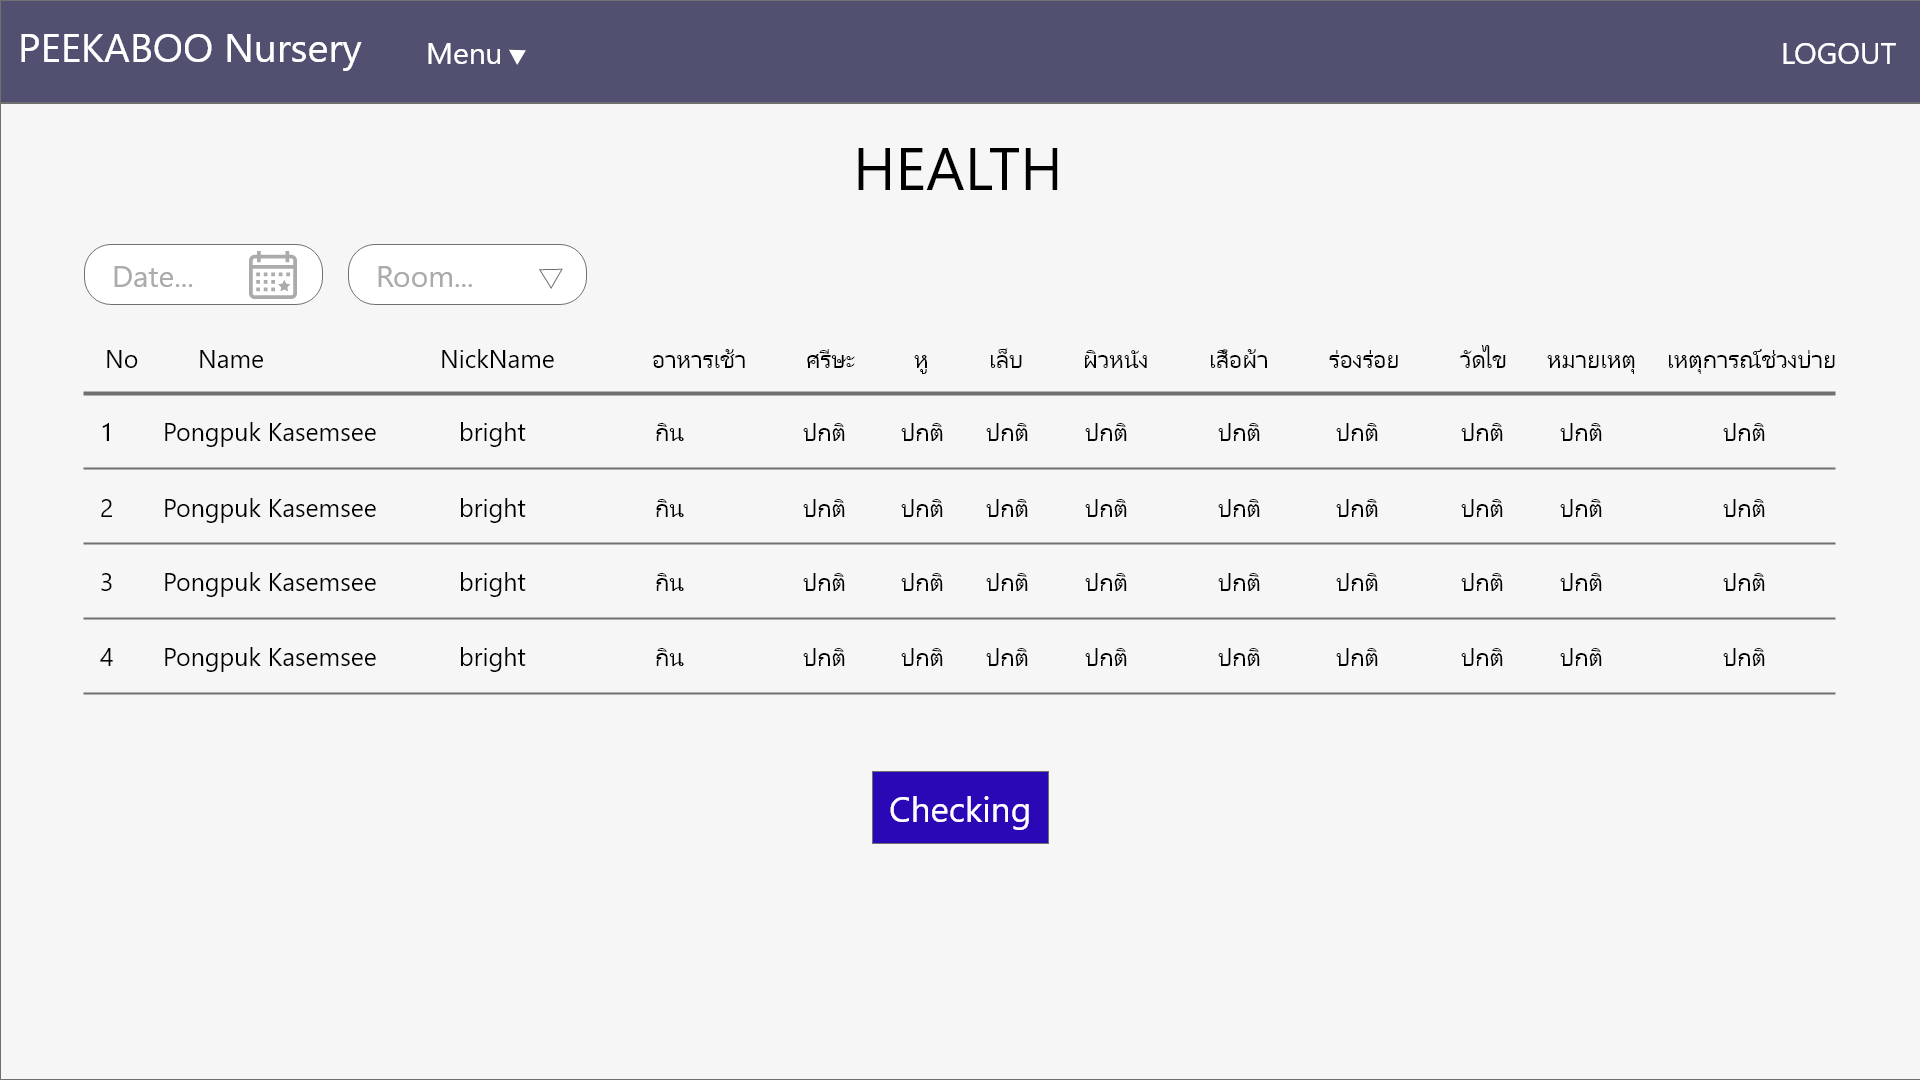
\includegraphics[width=\linewidth]{images/HealthPage.png}
  \end{center}
  \caption[Poem]{Health Page}
  \label{fig:Health}
  \end{figure}

\begin{figure}
  \begin{center}
  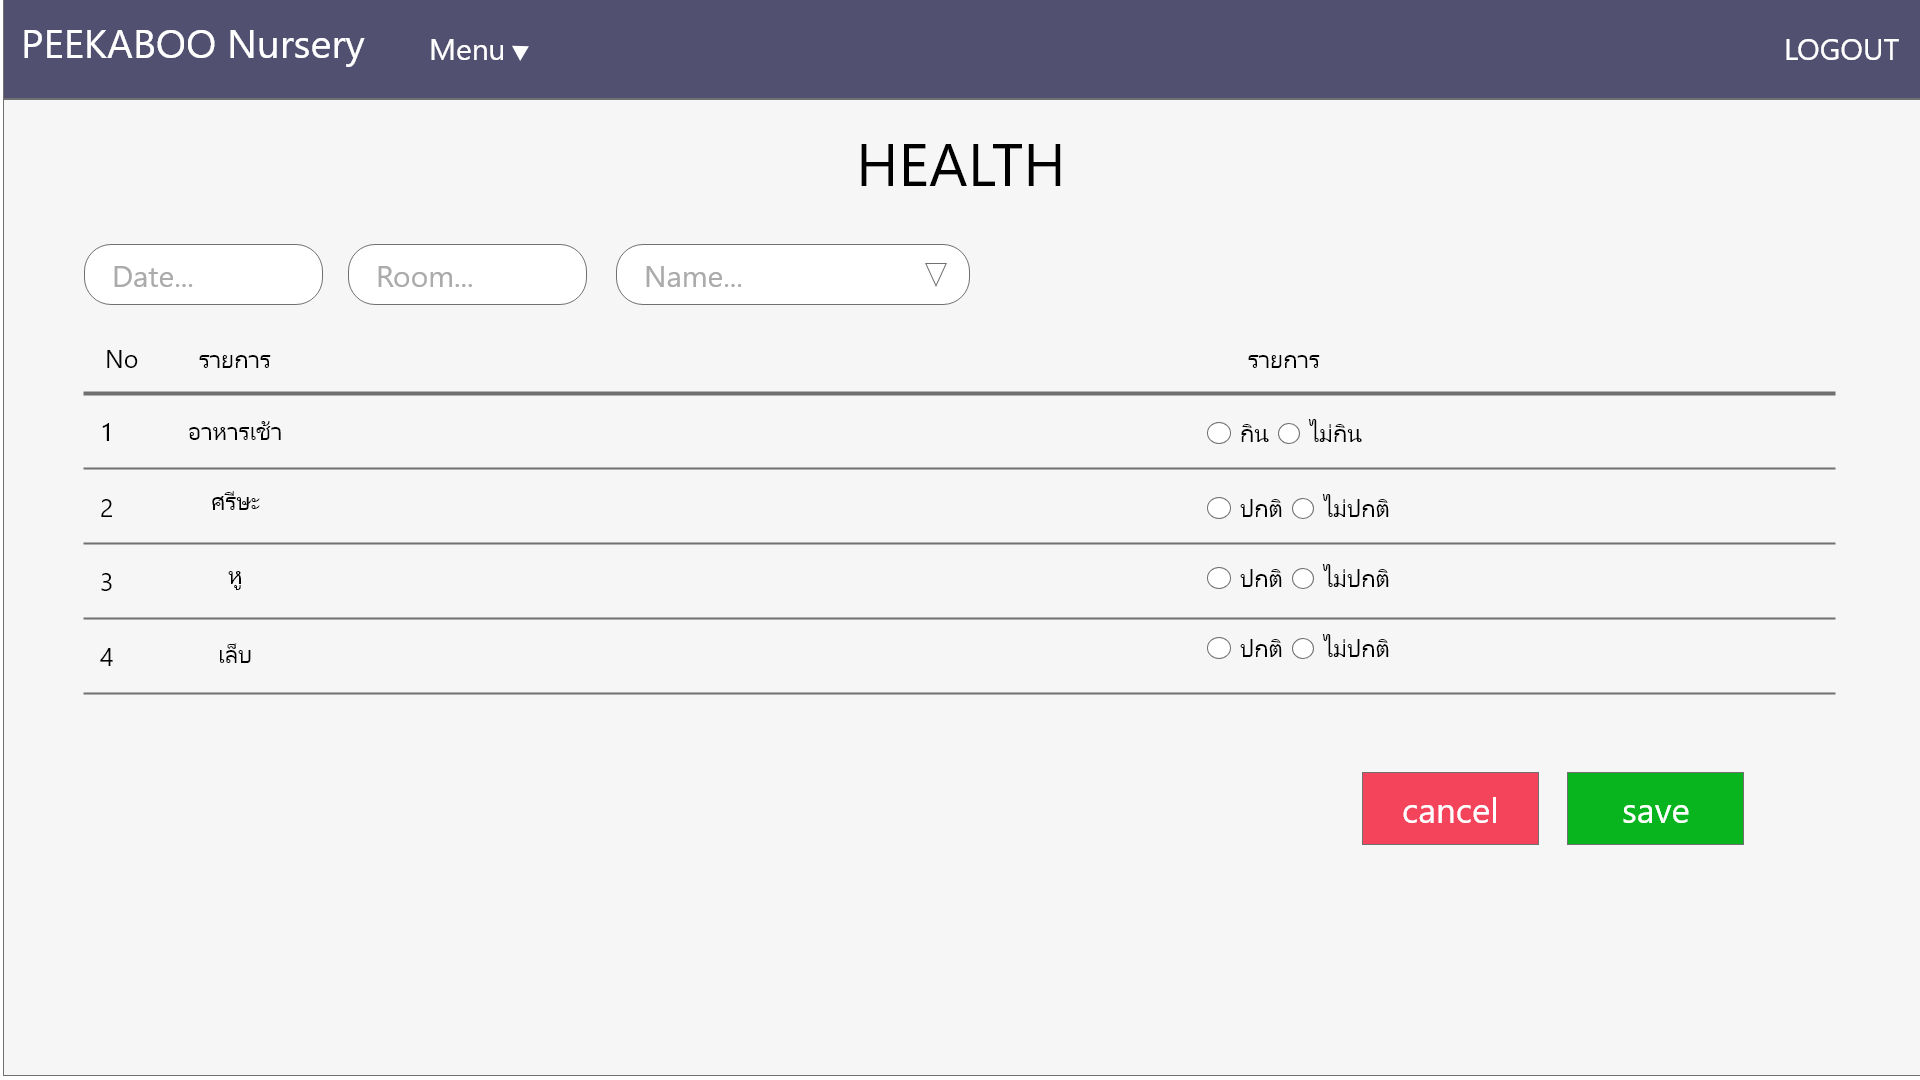
\includegraphics[width=\linewidth]{images/HealthPageChecking.png}
  \end{center}
  \caption[Poem]{Check Health Page}
  \label{fig:CheckHealth}
  \end{figure}

\begin{figure}
  \begin{center}
  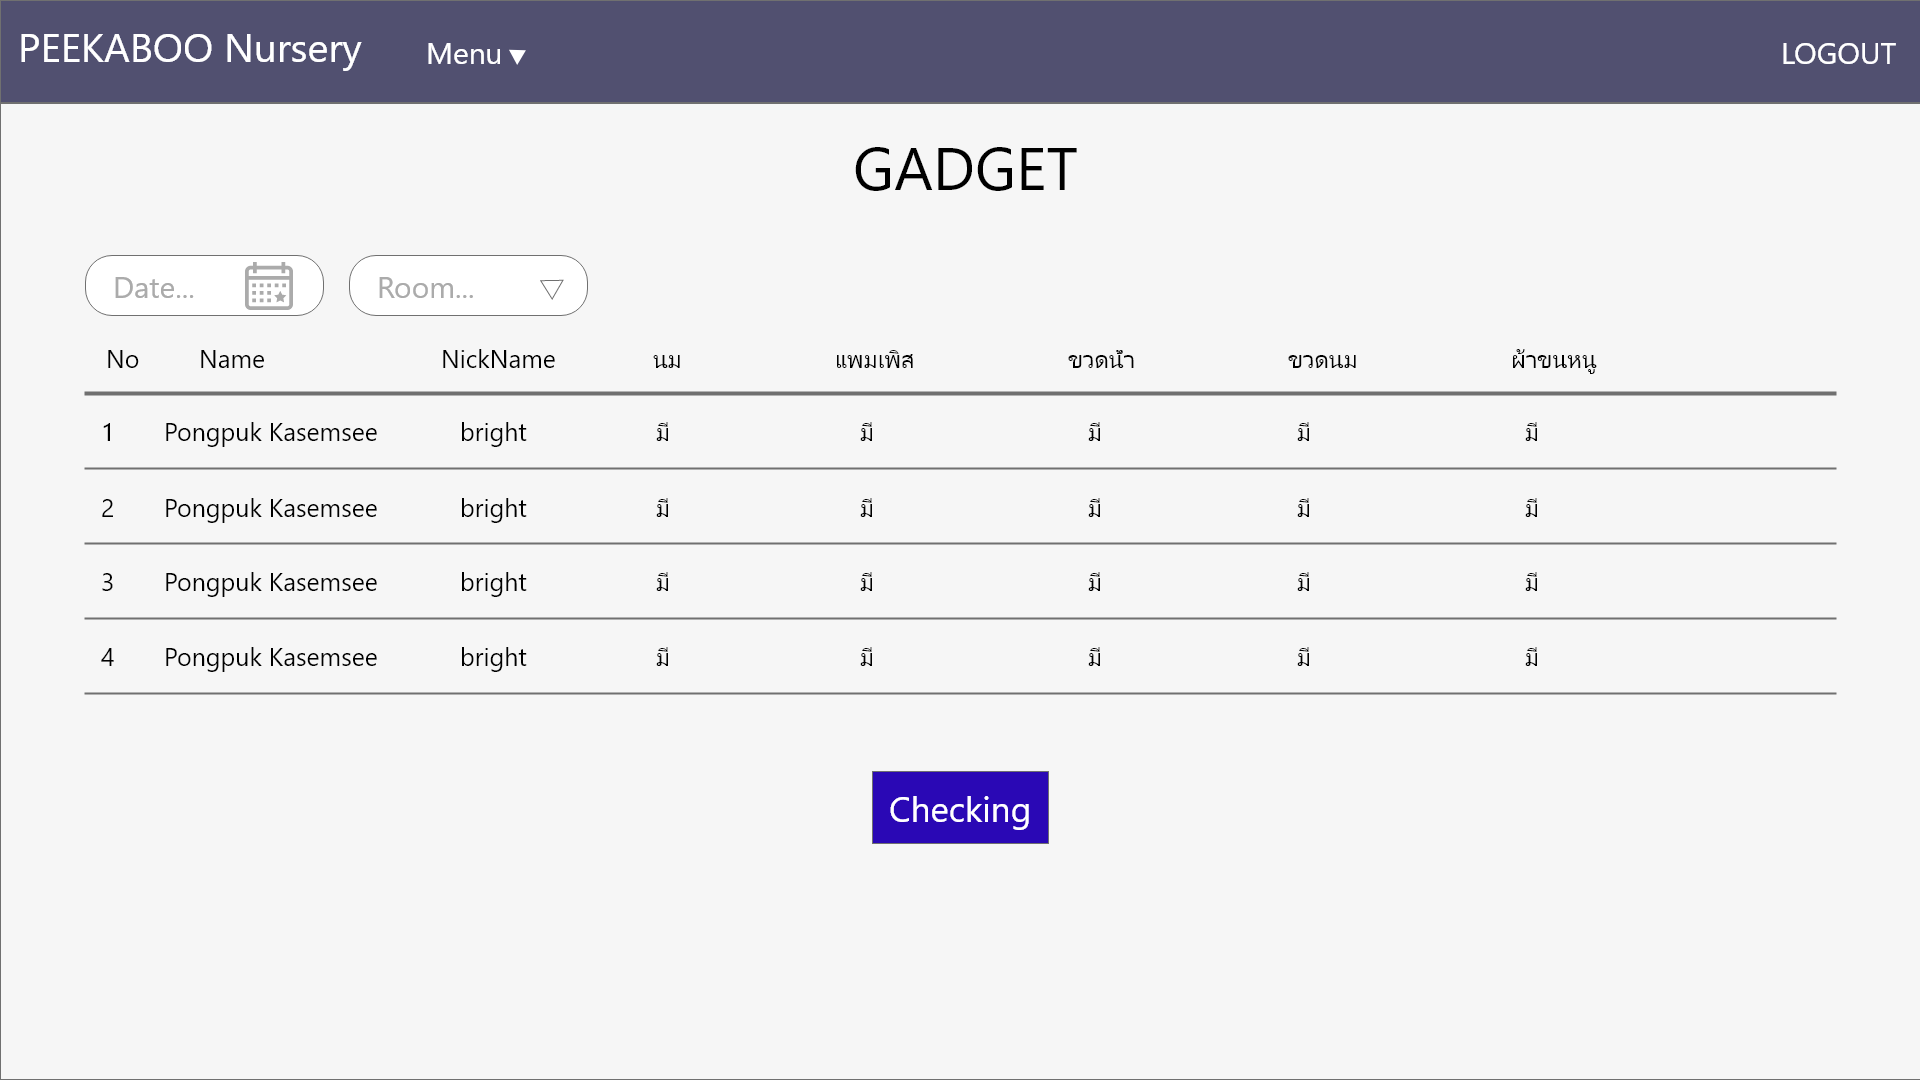
\includegraphics[width=\linewidth]{images/gadgetPage.png}
  \end{center}
  \caption[Poem]{gadget Page}
  \label{fig:Gadget}
  \end{figure}

\begin{figure}
  \begin{center}
  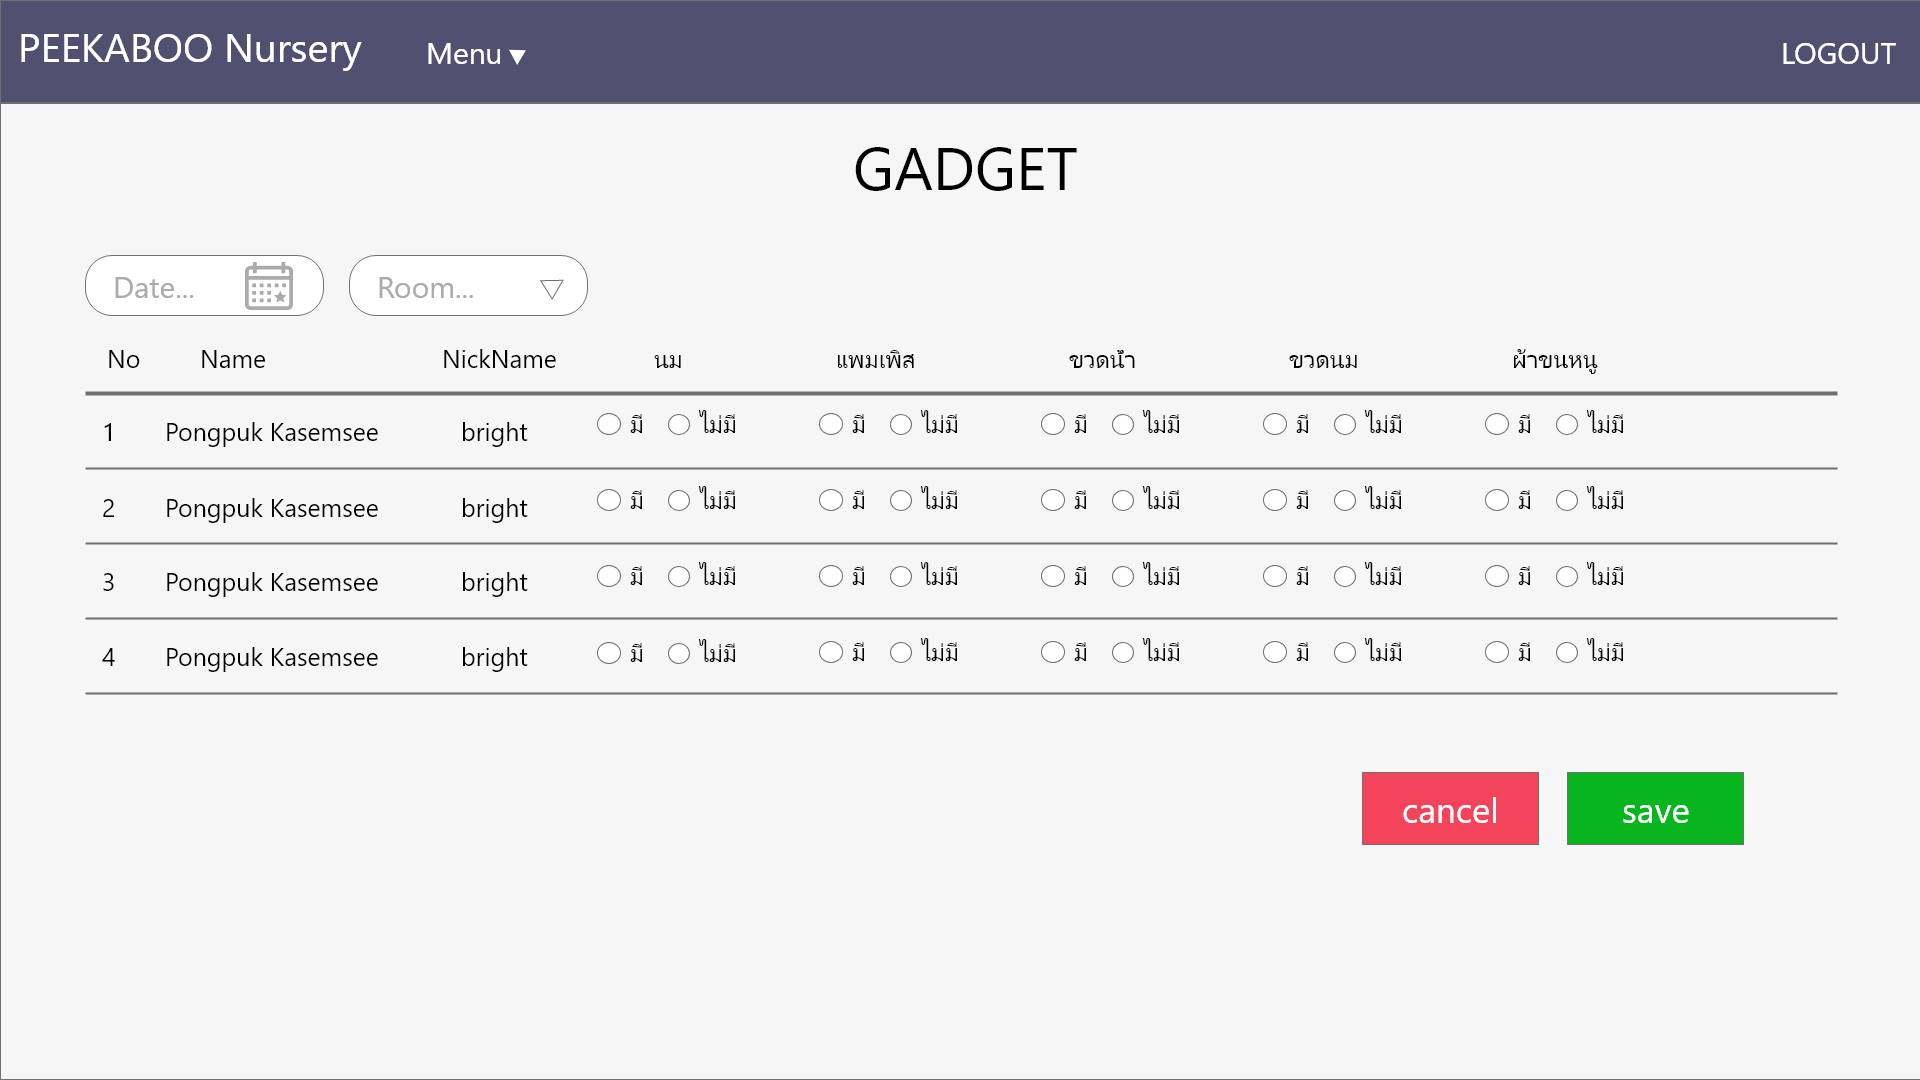
\includegraphics[width=\linewidth]{images/gadgetPageChecking.png}
  \end{center}
  \caption[Poem]{Check Gadget Page}
  \label{fig:CheckGadget}
  \end{figure}

\begin{figure}
  \begin{center}
  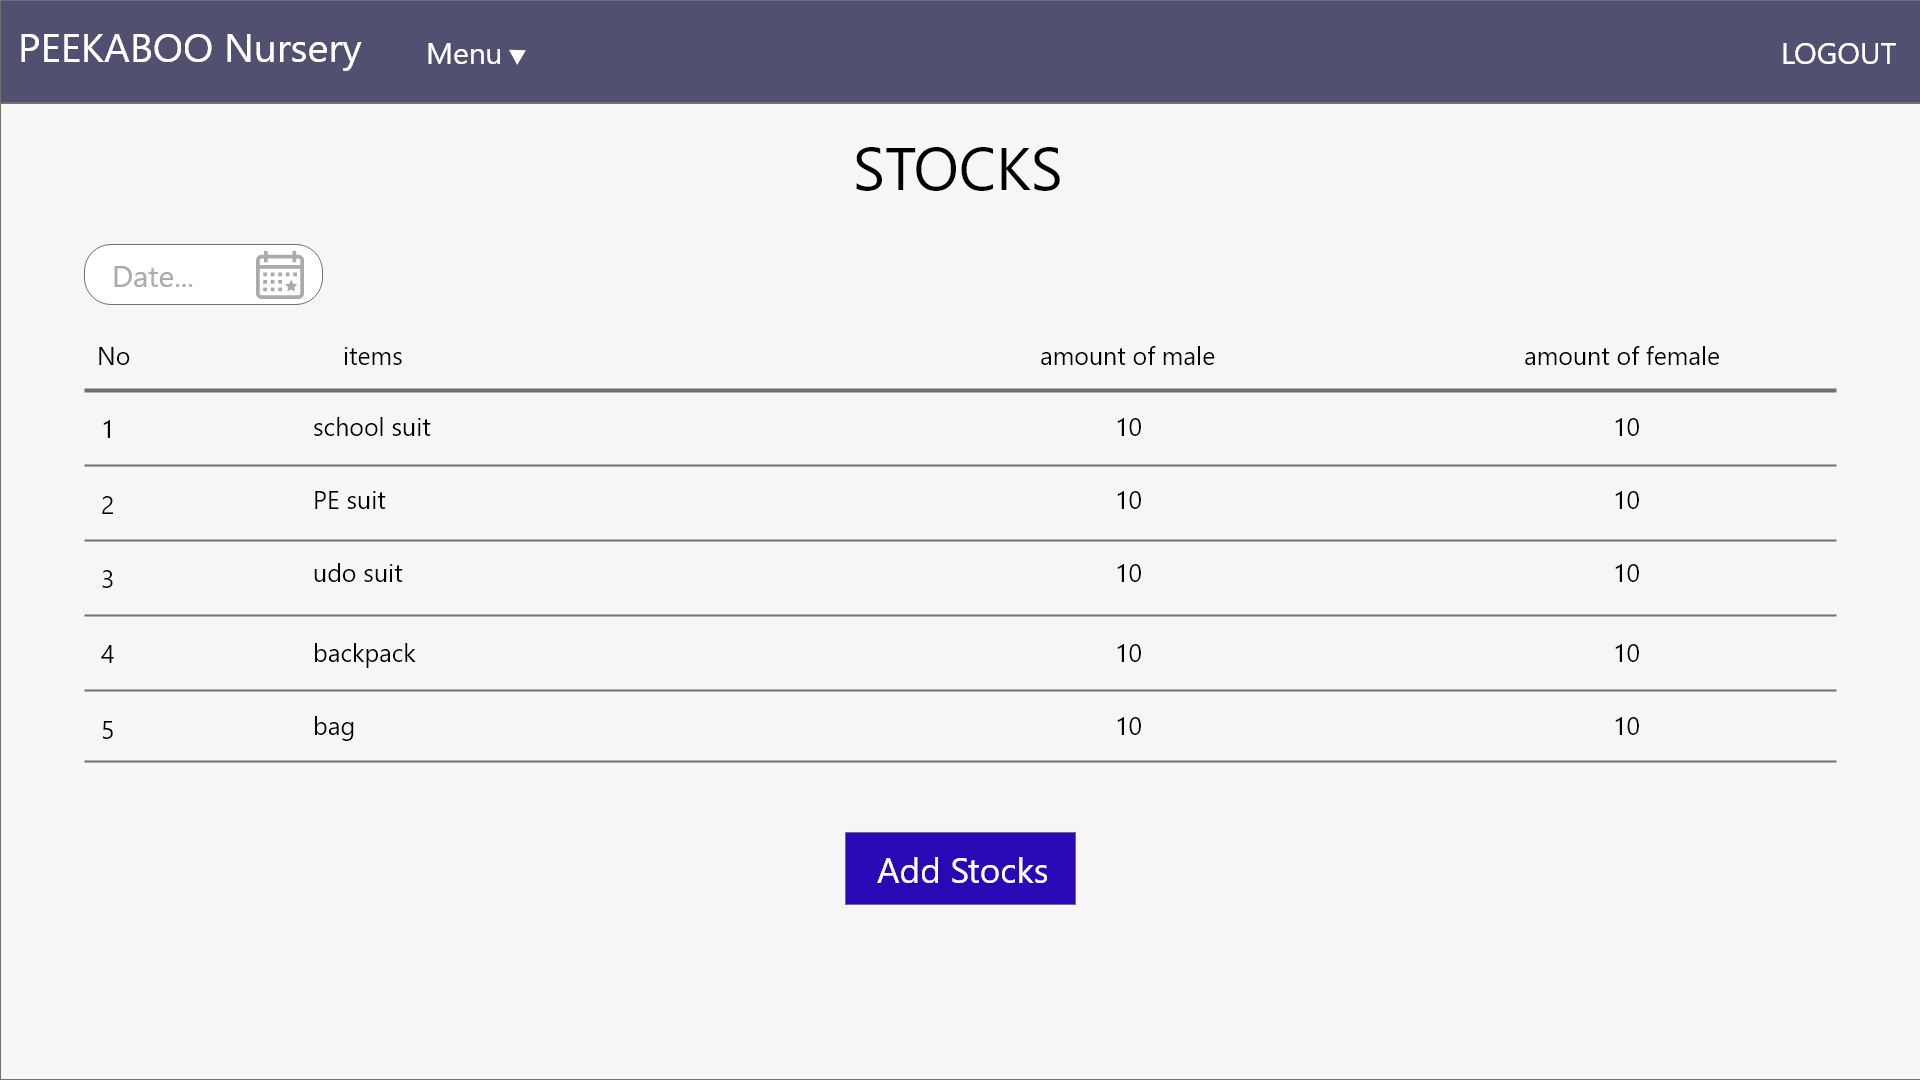
\includegraphics[width=\linewidth]{images/stockPage.png}
  \end{center}
  \caption[Poem]{Stock Page}
  \label{fig:Stock}
  \end{figure}

\begin{figure}
  \begin{center}
  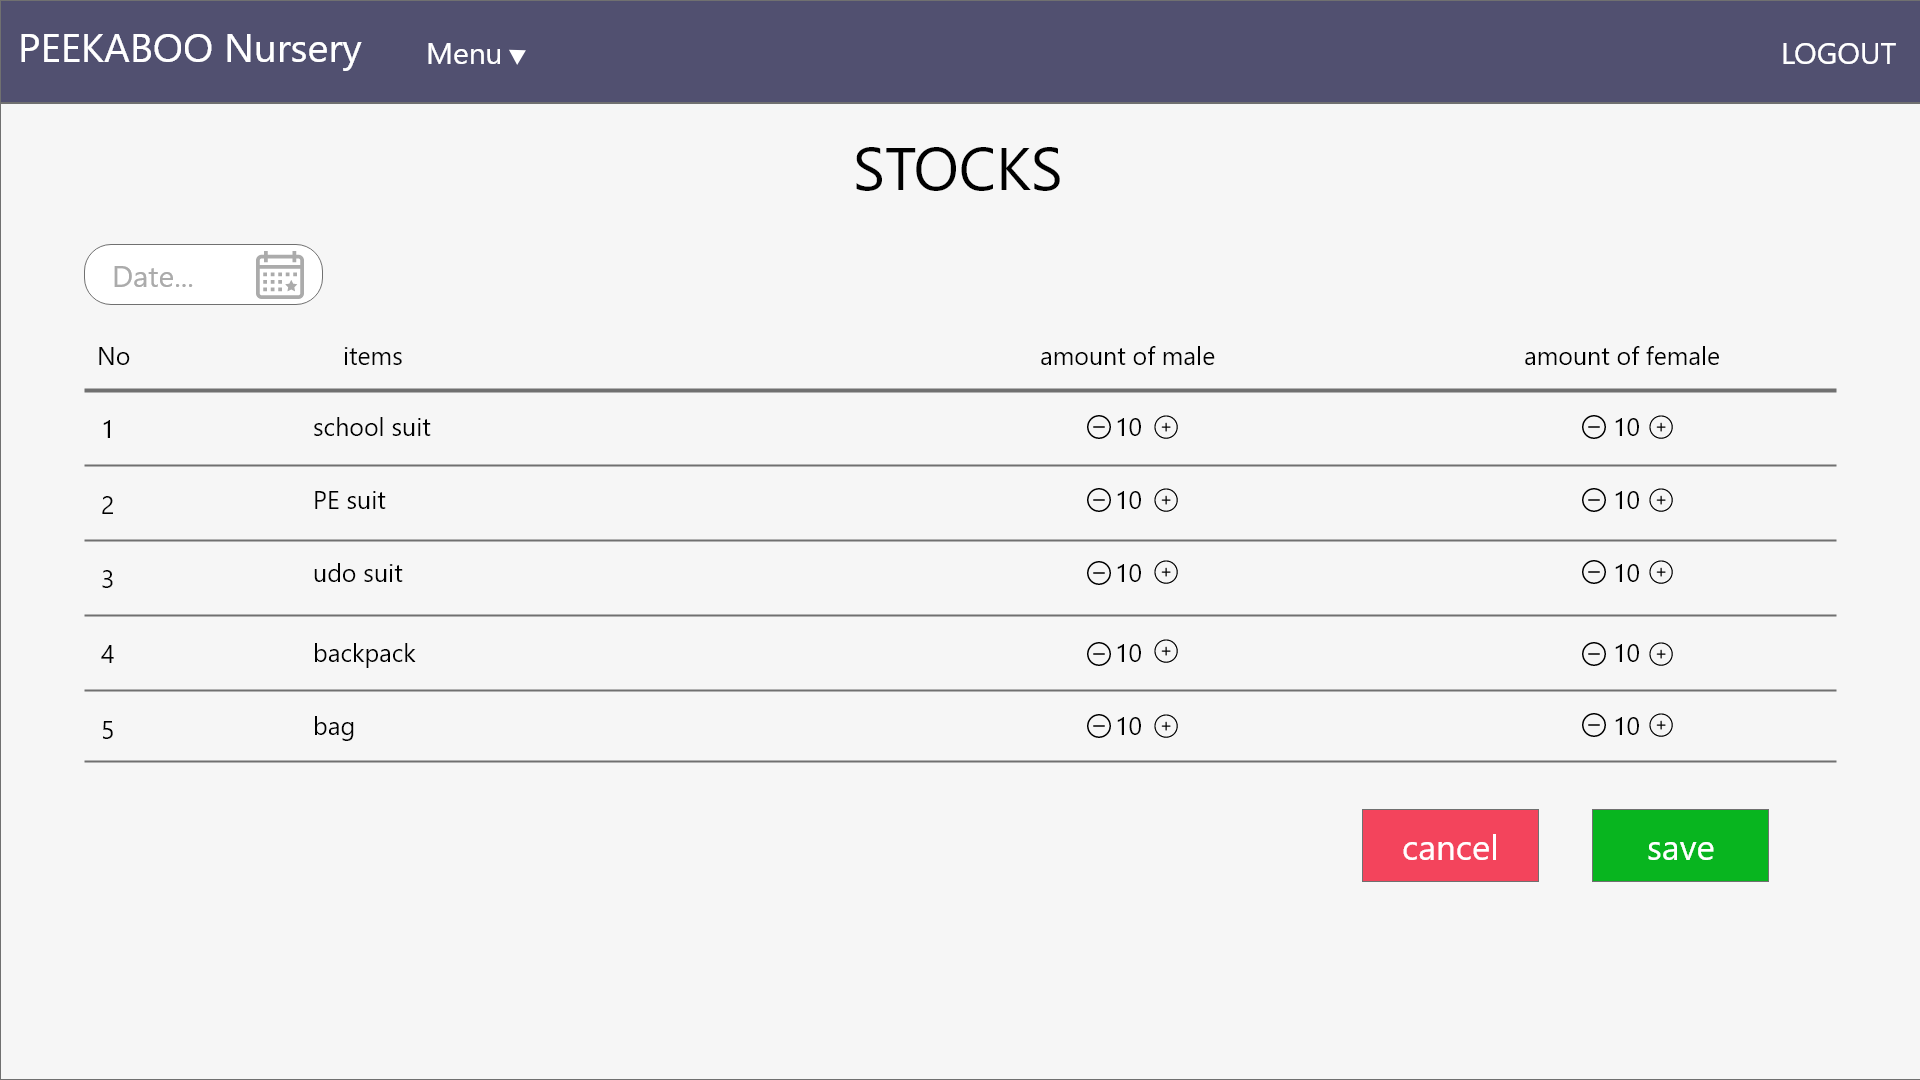
\includegraphics[width=\linewidth]{images/stockPageChecking.png}
  \end{center}
  \caption[Poem]{Check Stock Page}
  \label{fig:CheckStock}
  \end{figure}

\begin{figure}
  \begin{center}
  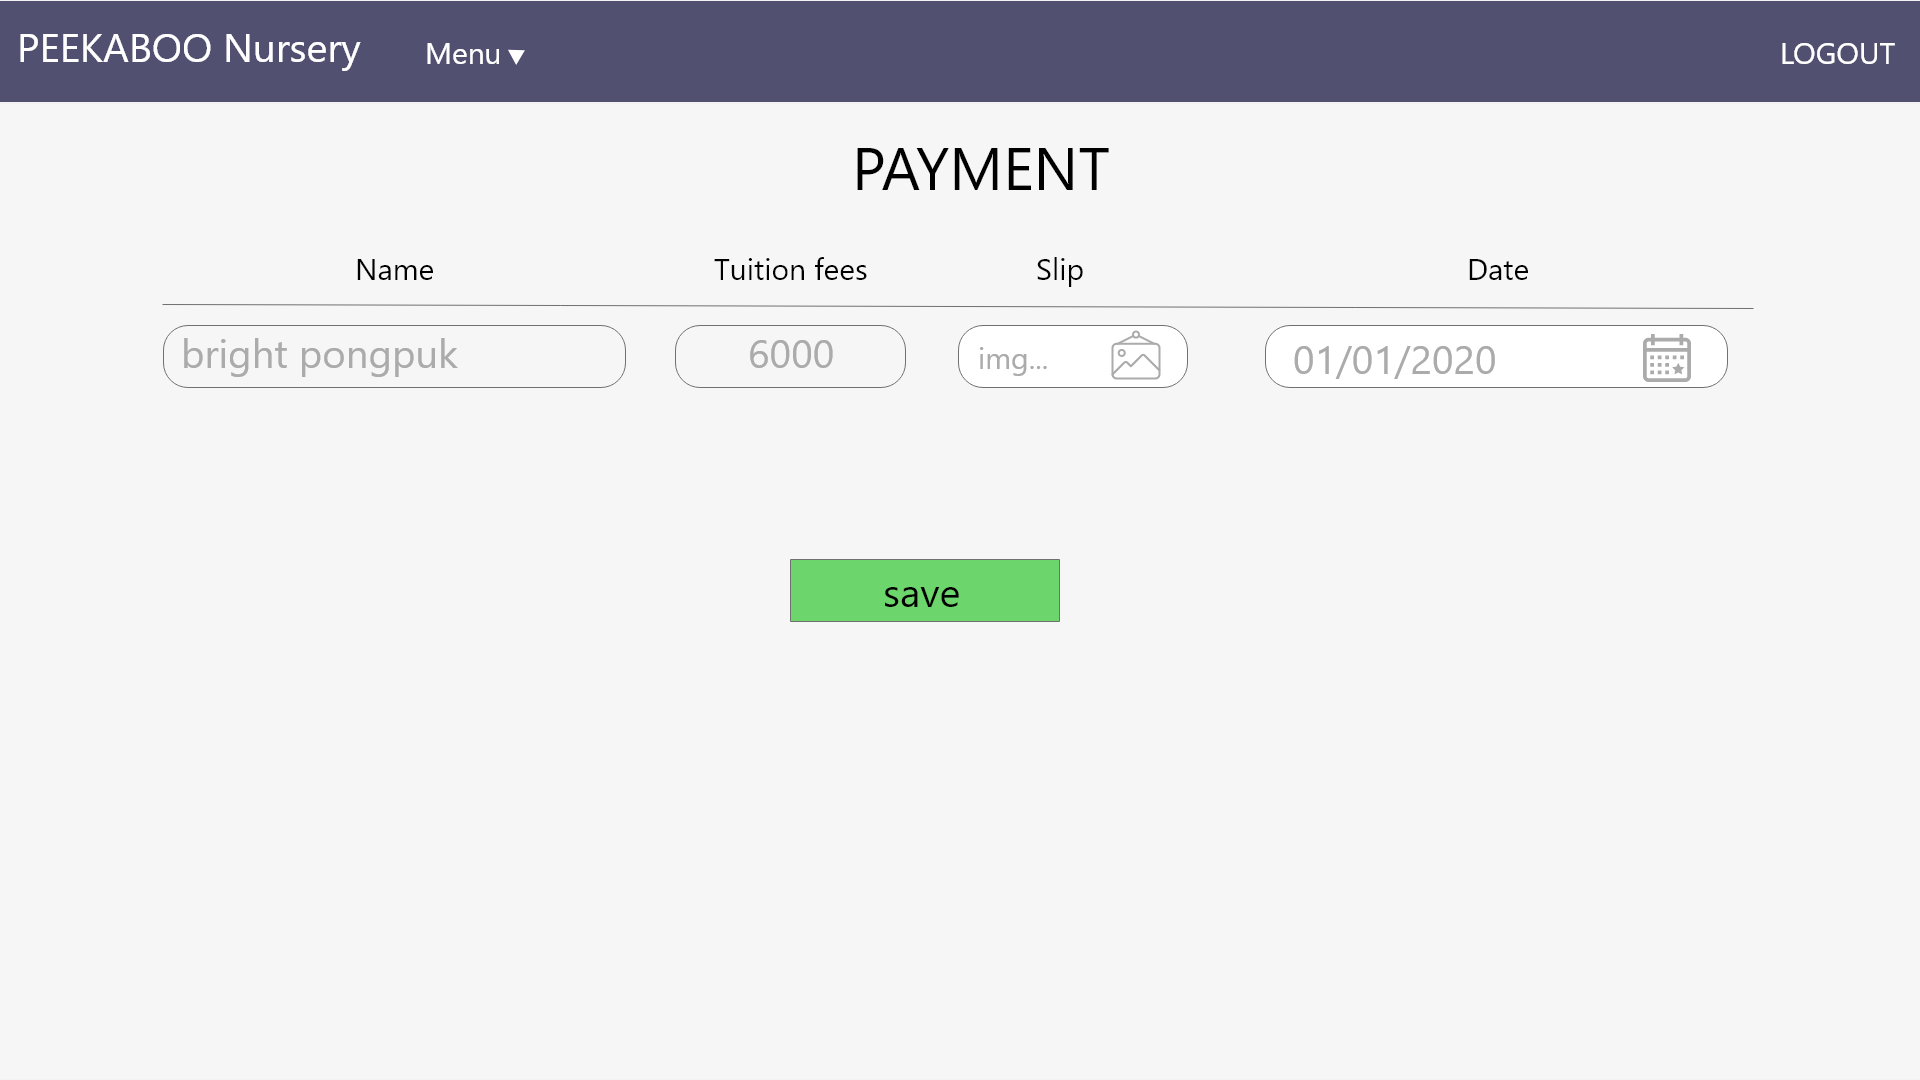
\includegraphics[width=\linewidth]{images/paymentPage.png}
  \end{center}
  \caption[Poem]{Payment Page}
  \label{fig:Payment}
  \end{figure}








\subsection{Architecture}

ระบบหลักๆที่ทางผู้พัฒนาใช้จะเป็นระบบแบบ Client-Server คือในทางฝั่ง Client จะใช้ React ในการพัฒนาแบบ Web-browser ให้ทางผู้ใช้ส่ง Requests มายังฝั่ง Server เพื่อที่จะทำงานต้องที่ผู้ใช้ต้องการ ซึ่งฝั่ง Server 
จะพัฒนาโดย Express.js ทางฝั่งนี้ก็จะ query ข้อมูลจากทางฐานข้อมูลที่เก็บไว้บน Mongodb Atlas เมื่อได้รับข้อมูลแล้วก็จะทำการส่ง Responses กลับไปยัง Client เพื่อให้ผู้ใช้สามารถทำงานในส่วนที่ต้องการได้ตามที่ต้องการ

\section{ขั้นตอนการดำเนินงาน}
\subsection{Discovery}
\begin{itemize}
  \item สำรวจและสอบถามปัญหาจากstakeholder
  \item นำปัญหาต่างหรือrequirementsมาวิเคราะห์
  \item สรุปผลแล้วนำrequirementsที่ได้จากการวิเคราะห์ไป  ทำต่อในขั้นตอนถัดไป
\end{itemize}

\subsection{Design}
\begin{itemize}
  \item ออกแบบหน้า UI/UX โดย Adobe XD
  \item ออกแบบฐานข้อมูลโดย Draw.io
  \item ออกแบบ
\end{itemize}

\subsection{Develop}
\begin{itemize}
  \item สร้าง Database
  \item เขียน Backend ตามที่ได้ Design มาในขั้นตอนก่อนหน้า
  \item เขียน Frontend แล้วทดสอบยิง Api ไปยังฝั่ง Backend
  \item เชื่อมโค้ด Frontend กับ Backend ผ่าน Api
\end{itemize}

\subsection{Testing}
